\documentclass[11pt,a4paper]{article}
\usepackage[utf8]{inputenc}
\usepackage[T1]{fontenc}
\usepackage[margin=1.7cm]{geometry}
\usepackage{graphicx}
\usepackage[hidelinks]{hyperref}
\usepackage{tabularx}
\usepackage{array}
\usepackage{enumitem}
\usepackage{setspace}

\setlength{\parindent}{0pt}
\setlength{\parskip}{6pt}
\setlength{\tabcolsep}{7pt}
\renewcommand{\arraystretch}{1.12}

\begin{document}
\pagestyle{empty}

\begin{center}
  \includegraphics[width=0.62\textwidth]{assets/logotextwbg50p.png}\\[0.4em]
  {\Large \textbf{Official Press Kit}}\\
  {\small Updated: 21 April 2026}
\end{center}

\vspace{0.35em}
\hrule
\vspace{0.9em}

\begin{minipage}[t]{0.65\textwidth}
  {\Large \textbf{Solm\aa ne}}\\[-0.15em]
  {\small Stylized as SOLM\AA NE}

  Portuguese alternative rock band from Braga, founded in 2024 by students from the University of Minho.

  \textbf{Genres:} Alternative Rock, Indie Rock, Acoustic Rock \\
  \textbf{Status:} Active \\
  \textbf{Booking:} \href{mailto:solmanebanda@gmail.com}{solmanebanda@gmail.com}
\end{minipage}
\hfill
\begin{minipage}[t]{0.32\textwidth}
  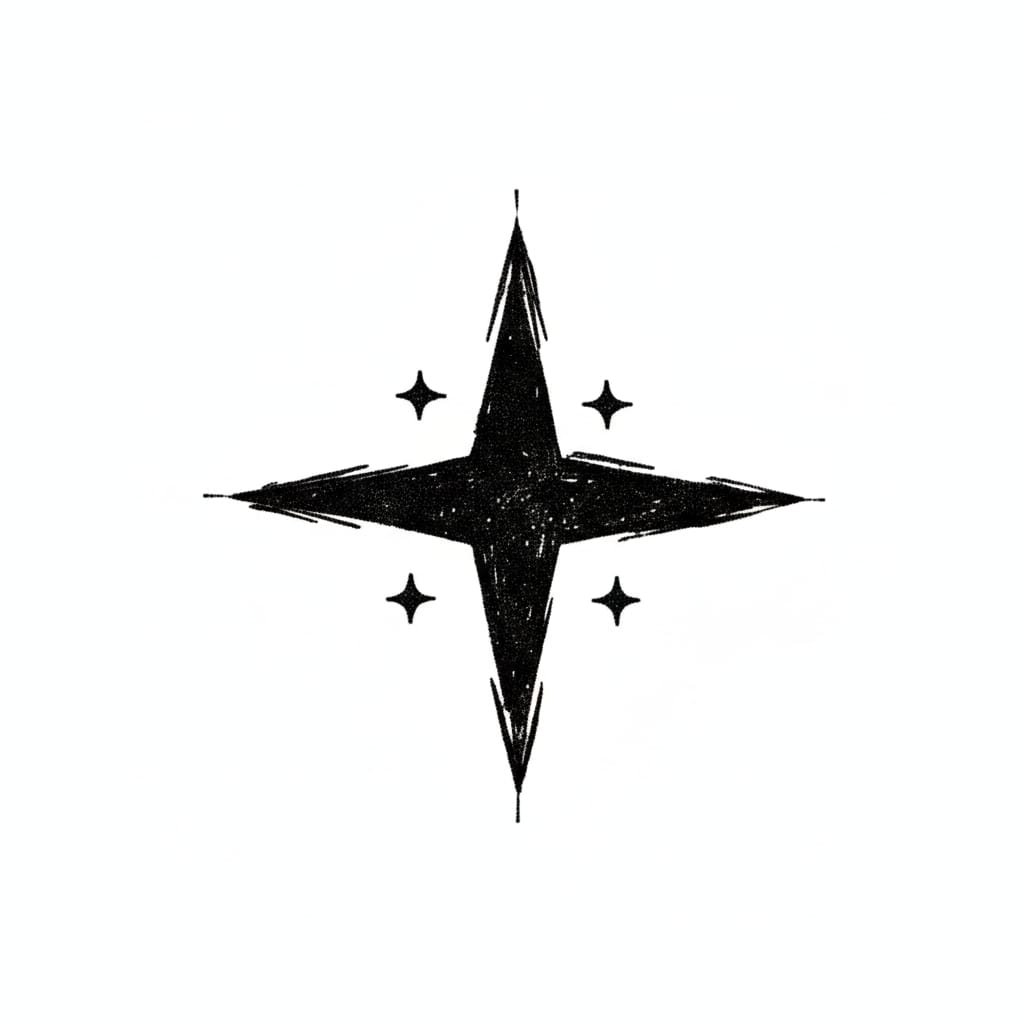
\includegraphics[width=\linewidth]{assets/0041678775_10.jpg}\\[-0.2em]
  {\footnotesize Live / rehearsal photo}
\end{minipage}

\vspace{0.9em}

\section*{Short Bio}
Solm\aa ne is a Portuguese independent rock band from Braga, formed in 2024. Built around a DIY spirit, the project combines melodic intensity, alternative textures and raw live energy. The band has become a regular presence in the university music circuit in Braga, with recurring performances at Okulto Bar and participation in AAUMinho Unplugged events.

\section*{Band Story}
The group was co-founded by Alexandre Fernandes, Nuno Leite, Bruno Coelho and Rodrigo Silva. Since its beginnings, Solm\aa ne has handled creation, production and online presence in-house. Their first release, \textit{Demos da Lage} (2025), captured the early sound of the band through an independent, experimental process.

\textbf{Founding members:} Alexandre Fernandes, Nuno Leite, Bruno Coelho, Rodrigo Silva.

\section*{Current Lineup}
\begin{itemize}[leftmargin=1.2em]
  \item Nuno Leite --- Vocals
  \item Alexandre Fernandes --- Drums
  \item David Ferreira --- Bass
  \item Rodrigo Silva --- Guitar
  \item Jo\~ao Ferreira --- Guitar
\end{itemize}

\textbf{Former member:} Bruno Coelho (Bass, co-founder).

\section*{Discography}
\textbf{EP: \textit{Demos da Lage}} (Independent, 26 April 2025)

\begin{tabularx}{\textwidth}{>{\raggedright\arraybackslash}p{0.08\textwidth} X >{\raggedleft\arraybackslash}p{0.12\textwidth}}
\textbf{\#} & \textbf{Track} & \textbf{Duration} \\
1 & Dance With the Devil & 3:23 \\
2 & Out of Reach & 3:43 \\
3 & Balada (Lose the Light) & 6:00 \\
\end{tabularx}

\textbf{Total runtime:} 13:06

\textbf{Recording credits (EP):} Vocals --- Nuno Leite; Drums --- Alexandre Fernandes; Bass --- Bruno Coelho; Guitars --- Rodrigo Silva and Jo\~ao Ferreira. Cover artwork by Nuno Leite.

\section*{Live and Media Highlights}
\begin{itemize}[leftmargin=1.2em]
  \item Frequent performances in Braga's university music circuit.
  \item Recurring live appearances at Okulto Bar (Braga).
  \item Participation in AAUMinho Unplugged (2025 and 2026).
  \item 2025 Unplugged participation included collaboration with Mafalda Martins.
  \item Podcast interview available on YouTube.
\end{itemize}

\section*{Official Links}
\begin{tabularx}{\textwidth}{>{\raggedright\arraybackslash}p{0.2\textwidth} X}
Website & \href{https://solmaneband.github.io/}{solmaneband.github.io} \\
Spotify & \href{https://open.spotify.com/artist/0XYxjDhjXN9VEgTs7Z59iq}{Artist Profile} \\
Bandcamp & \href{https://solmane.bandcamp.com/album/demos-da-lage}{Demos da Lage} \\
Apple Music & \href{https://music.apple.com/lu/artist/solmane/1673074844}{Artist Profile} \\
Amazon Music & \href{https://music.amazon.com/albums/B0FJY9FCXG}{Demos da Lage} \\
Instagram & \href{https://www.instagram.com/solmaneofficial/}{@solmaneofficial} \\
YouTube & \href{https://www.youtube.com/@Solmaneofficial}{@Solmaneofficial} \\
Facebook & \href{https://www.facebook.com/profile.php?id=61585087408800}{Official Page} \\
Podcast Interview & \href{https://www.youtube.com/watch?v=gz7kYAouGes}{Watch on YouTube} \\
\end{tabularx}

\section*{Contact}
For bookings, press requests and collaboration opportunities:
\begin{itemize}[leftmargin=1.2em]
  \item Email: \href{mailto:solmanebanda@gmail.com}{solmanebanda@gmail.com}
  \item Press kit file: \href{https://solmaneband.github.io/assets/presskit.pdf}{solmaneband.github.io/assets/presskit.pdf}
\end{itemize}

\vfill
\begin{center}
  {\small Solm\aa ne \textbar{} Press Kit \textbar{} 2026}
\end{center}

\end{document}
